\documentclass[
	12pt,
	BCOR=5mm,
	DIV=12,
	headinclude=on,
	footinclude=off,
	parskip=half,
	bibliography=totoc,
	listof=entryprefix,
	toc=listof,
	numbers=noenddot,
]{scrreprt}

\usepackage[ngerman]{babel}
\usepackage[german=quotes]{csquotes}
\usepackage{microtype}
\usepackage{color}
\usepackage[german]{varioref}
\usepackage{hyperref}
\usepackage{amsmath}
\usepackage{amsthm}
\usepackage{marvosym}
\usepackage{lmodern}
\usepackage{graphicx}

\usepackage{float}

\MakeOuterQuote{"}

% Uncomment the next three lines for author-year-style with footnotes (Chicago)
\usepackage[backend=biber, autocite=footnote, style=authoryear, dashed=false]{biblatex}
% \AdaptNoteOpt\footcite\multfootcite 
% \AdaptNoteOpt\autocite\multautocite

\DefineBibliographyStrings{ngerman}{  %Change u.a. to et al. (german only!)
	andothers = {{et\,al\adddot}},
}
\setlength{\bibparsep}{\parskip}
\addbibresource{references.bib}

\hypersetup{
    linktoc=all,
    colorlinks=true,
    linkcolor=black,
    citecolor=black,
    urlcolor=black
}
\theoremstyle{definition}
\newtheorem{example}{Beispiel}
\pagestyle{headings}

\newcommand{\TitelDerArbeit}[1]{\def\DerTitelDerArbeit{#1}\hypersetup{pdftitle={#1}}}
\newcommand{\AutorDerArbeit}[1]{\def\DerAutorDerArbeit{#1}\hypersetup{pdfauthor={#1}}}
\newcommand{\Firma}[1]{\def\DerNameDerFirma{#1}}
\newcommand{\Kurs}[1]{\def\DieKursbezeichnung{#1}}

\RequirePackage[automark,headsepline,footsepline]{scrpage2}
\pagestyle{scrheadings}
\renewcommand*{\pnumfont}{\upshape\sffamily}
\renewcommand*{\headfont}{\upshape\sffamily}
\renewcommand*{\footfont}{\upshape\sffamily}
\renewcommand{\chaptermarkformat}{}
\RedeclareSectionCommand[beforeskip=0pt]{chapter}
\clearscrheadfoot

%\ifoot[\rule{0pt}{\ht\strutbox+\dp\strutbox}DHBW Mannheim]{\rule{0pt}{\ht\strutbox+\dp\strutbox}DHBW Mannheim}
%\ofoot[\rule{0pt}{\ht\strutbox+\dp\strutbox}\pagemark]{\rule{0pt}{\ht\strutbox+\dp\strutbox}\pagemark}

\ohead{\headmark}


\TitelDerArbeit{Die Inflationstheorie der Monetaristen -\\ Eine Betrachtung der Quantitätstheorie}
\AutorDerArbeit{Aaron Schweig}
\Firma{Hays AG}
\Kurs{WWI18SEC}

\begin{document}
\pagenumbering{roman}
\begin{titlepage}
    \begin{minipage}{\textwidth}
            \vspace{-2cm}
            \noindent 
            % \includegraphics[scale=0.71]{img/firmenlogo.jpg} 
            \hfill   
\includegraphics{img/logo.jpg}
    \end{minipage}
    \vspace{1em}
    \sffamily
    \begin{center}
        \textsf{\large{}Duale Hochschule Baden-W\"urttemberg\\[1.5mm] Mannheim}\\[2em]
        \textsf{\textbf{\Large{}Hausarbeit}}\\[3mm]
        \textsf{\textbf{\DerTitelDerArbeit}} \\[1.5cm]
        \textsf{\textbf{\Large{}Studiengang Wirtschaftsinformatik}\\[3mm] \textsf{Studienrichtung Software Engineering}}
        
        \vspace{3em}
        % \textsf{\Large{Sperrvermerk}}
    \vfill
    
    \begin{minipage}{\textwidth}
    
    \begin{tabbing}
        Wissenschaftlicher Betreuer: \hspace{0.85cm}\=\kill
        Dozent: \> Prof. Dr. Rüdiger Funk \\[1.5mm]
        Verfasser: \> \DerAutorDerArbeit \\[1.5mm]
        Matrikelnummer: \> 6161622 \\[1.5mm]
        Firma: \> \DerNameDerFirma  \\[1.5mm]
        Kurs: \> \DieKursbezeichnung \\[1.5mm]
        Studiengangsleiter: \> Prof. Dr. Sebastian Ritterbusch  \\[1.5mm]
        % \> +49 151 / 123 456 \\[1.5mm]
        Bearbeitungszeitraum: \> 18.05.2020 -- 20.07.2020
    \end{tabbing}
    \end{minipage}
    
    \end{center}
    
    \end{titlepage}

\tableofcontents

\listoffigures


\chapter{Einleitung}

\pagenumbering{arabic}
\ihead{\chaptername~\thechapter}

\marginpar{Einleitung noch anpassen, wenn alles fertig ist}
In der folgenden Arbeit wird die Inflationtheorie der Monetaristen näher beleuchtet. Dabei wird versucht zuerst eine allgemeine Basis zu schaffen, indem zuerst Definitionen sowohl der Infaltion selbst, als auch der Geldmenge als weiteren Bestandteil der Theorie aufzustellen. Im folgenden wird dann die Quantitätstheorie sowie die Quantitätsformel erläutert. Hierbei wird vorallem auf die besonderheiten bei der Ableitung der Formel aus der Theorie eingegangen, sowie auf die Annahmen, welche in diesem Rahmen getroffen werden. Im Anschluss wird dann untersucht, inwiefern die Quantitätsformel als Repräsentant der Inflationstheorie in der heutigen Zeit anwendbar, oder nicht anwendbar ist, was letztendlich zu einem Fazit mit einem Vergleich zwischen der Quantitätstheorie und alternativen Theorien zusammengeführt wird.

Der Monetarismus ist eine wirtschaftstheoretische Konzeption, welche im Gegensatz zu dem nachfrageorientierten Keynesianismus steht. Für einen Monetaristen steht die Regulierung der Geldmenge die wichtigste Stellschraube in der in der Steuerung des Wirtschaftsablaufs dar. Es gilt also die Devise:

\begin{center}
    "Money matters" - Es kommt auf die Geldmenge an.
\end{center}

Der Monetarismus wurde geprägt von Ives Fisher, welcher in seiner Quantitätstheorie formuliert.

\chapter{Die Quantitätstheorie}

\section{Geschichte der Quantitätstheorie}
Bereits im 16. Jahrhundert war die Idee der Quantitätstheorie vorhanden. Es wurde argumentiert, dass der Zufluss an Gold und Silber, durch neue Handelsrouten mit Asien, die Preise in Europa beeinflusste. Im Mittelalter wurde also bereits postuliert, dass die Menge der Zahlungsmittel einen Einfluss auf die Preisbildung hat \autocite{Woll1977}.

Diese Gedanken wurden dann, Anfang des 19. Jahrhunderts, wissenschaftlich bearbeitet und Ökonomen begannen, eine allgemeine Theorie zur Verhaltensbestimmung des Preises auf Basis der zur Verfügung stehenden Zahlungsmittel aufzustellen.\\
Im Jahr 1911 formulierte der Ökonom \textbf{Irving Fisher} in seiner Arbeit \enquote{The Purchasing Power of Money} die erste Version dessen, was allgemein als Quantitätstheorie bekannt ist. Der wohl bekannteste Vertreter der Neo-Quantitätstheorie ist der amerikanische Ökonom \textbf{Milton Friedman}. Die Anhänger dieser Theorie sind auch als \textbf{Monetaristen} bekannt.

Mit \textbf{John Maynard Keynes} findet die Quantitätstheorie einen ihrer schärfsten Kritiker, welcher behauptet, dass die Möglichkeit der Einflussnahme einer Zentralbank auf die Realwirtschaft durch Steuerung der Geldmenge nicht möglich sei. Seine nachfrageorientierte Inflationstheorie findet heute noch in Form des Keynesianismus eine große Popularität.

\section{Allgemeine Quantitätsgleichung}

Die Quantitätstheorie vertritt den Ansatz, dass durch Steuerung der Geldmenge die Realwirtschaft beeinflusst werden kann. Genauer wird behauptet, dass sich der Preis verändert. \\
Mithilfe der Inflation, einer Erhöhung der Geldmenge, soll ein höherer Preis erreicht werden. Durch Deflation, einer Verkleinerung der Geldmenge, soll ein niedrigerer Preis erzielt werden. Diese Idee führt so folgender Gleichung:
\begin{equation}
    \tag{Allg. Quantitätsgleichung}
    M \cdot V = T \cdot P
\end{equation}\label{allg. Q-Formel}

Die allgemeine Quantitätsgleichung beschreibt eine Identität zwischen dem Produk der Geldmenge $M$ und er Geldumlaufgeschwindigkeit $V$, sowie dem Produkt der Anzahl aller Transaktionen $T$ und dem durchschnittlichen Preis $P$ dieser Transaktionen. Um die Identität etwas deutlicher zu machen, können die beiden Seiten der Gleichung folgendermaßen interpretiert werden:

\subsubsection*{Das Produkt $M \cdot V$:}
Die Geldmenge multipliziert mit der Geldumlaufgeschwindigkeit stellt nichts anderes dar, als die \enquote{Summe aller Zahlungen} in einer Realwirtschaft.

\subsubsection*{Das Produkt $T \cdot P$:}
Hierbei handelt es sich um die \enquote{Summe der Werte aller Käufe}.

\subsubsection*{Interpretation der Gleichung}
Betrachtet man die beiden Interpretationen der Identität \vref{allg. Q-Formel} stellt man fest, dass die Aussage die \enquote{Summe aller Zahlung ist gleich der Summe der Werte aller Käufe} im Rahmen einer volkswirtschaftlichen Betrachtung ohne Ausnahme bejaht werden kann. Es handelt sich bei der Identität also um eine \textbf{Tautologie}.

Um nun diese Feststellung in der realwirtschaftlichen Betrachtung nutzen zu können, müssen die einzelnen Komponenten der Formel eine Bedeutung erhalten. Um z.B. die Geldmenge $M$ zu bestimmen, können bereits bekannte Größen für Geldmenge, $M_0$, $M_1$,$M_2$ oder $M_3$, herangezogen werden. Es spielt vorerst keine Rolle, welche Geldmenge betrachtet wird, sofern die Wahl der anderen Komponenten der Gleichung mit Beachtung dieser Entscheidung erfolgt.

Versucht man, die anderen Faktoren zu bestimmen, so lassen sich Probleme bei der Messbarkeit dieser Größen feststellen. Einen Wert für die Anzahl der Transaktionen $T$ festzulegen ist bei einer volkswirtschaftlichen Gesamtbetrachtung sehr schwierig. Die meisten Transaktionen, also Vorgänge, bei denen Geld zwischen zwei Parteien ausgetauscht wird, in einer Volkswirtschaft sind Finanztransaktionen.

Zusätzlich dazu ist es quasi unmöglich einen Wert für die Umlaufgeschwindigkeit $V$ zu bestimmen. Hierbei muss zunächst darauf geachtet werden, dass die richtige Menge an Vorgängen betrachtet wird, welche abhängt von der Wahl der Geldmenge $M$. Es ist nicht möglich alle Vorgänge zu zählen, in denen das Geld in Umlauf gebracht wird.
Ebenfalls ist es aus den selben Gründen nicht möglich einen exakten durchschnittlichen Preis $P$ zu bestimmen, da zur Berechnung eines Durchschnitts sowohl Anzahl, als auch die Messgröße (hier der Preis einer Transaktion) bekannt sein muss.

Die Gleichung \vref{allg. Q-Formel} stellt also als Tautologie einen wahren Zusammenhang dar. Beim Versuch diesen nutzbar zu machen und in der Praxis anzuwenden, werden Probleme deutlich, die zuerst gelöst werden müssen.

\section{Herleitung der eigentlichen Quantitätsgleichung}
\marginpar{Ab 2.3 noch weiterlesen}
Im weiteren Entwicklungsverlauf der Theorie wurde versucht die Formel so zu spezifizieren, dass sie zugänglicher wird. Gleichzeitig sollte erreicht werden, dass auch mit Werten gearbeitet werden kann, welche im Rahmen einer Volkswirtschaft bekannt sind.

Die Einschränkung, die diese Spezifizierung ermöglicht, betrifft das Transaktionsvolumen $T$. Anstelle \textbf{aller} Transaktionen werden innerhalb der Formel nur die Transaktionen betrachtet, welche eine Auswirkung auf das BIP $Y$ haben. Dabei fällt also der oben bereits erwähnte größte Anteil der Transaktionen, nämlich die Finanztransaktionen, weg. Das BIP ist eine gut messbare und bekannte Größe innerhalb einer Volkswirtschaft. Allerdings gilt es jetzt, da es sich bei der Gleichung um eine Identität handelt, auch die Gegenseite anzupassen, um sicherzustellen, dass es sich bei der Gleichung um eine wahre Aussage handelt. Die betrachtete Geldmenge ist bereits bekannt und auch Messbar, wie bereits oben festgestellt werden konnte. Also gilt es nun zu versuchen die Umlaufgeschwindigkeit $V$ näher bestimmen zu können. Da auch diese Abhängig von der Anzahl und Art der Transaktion ist wird nun versucht die Umlaufgeschwindigkeit des Geldes auf Basis des BIP zu bestimmten.

Dies führt zu einer neuen Formel: 

$$ M \cdot V_Y = Y \cdot P$$\label{QFormel}
In der Literatur wird die Formel dabei auch ohne den Index bei der Umlaufgeschwindigkeit geschrieben.

$$ M \cdot V = Y \cdot P$$

Dies verleitet einen unerfahrenen Ökonomen oftmals dazu sich nicht klarzumachen, dass es sich hierbei nur um die durchschnittliche Umlaufgeschwindigkeit der Geldmenge, welche \textbf{wirksam auf das BIP} sind, handelt.

Eine weitere Annahme, welche bereits Eingangs angesprochen wurde, ist, dass es sich bei der Umlaufgeschwindigkeit $V_Y$ um einen (annähernd) konstanten Wert $\overline{V}_Y$ handelt. Die Bedeutung dieser Annahme kann am besten anhand eines Beispiels aufgezeigt werden.

\begin{example}[Konstante Umlaufgeschwindigkeit]
    Man nehme einen Haushalt $H$ mit einer angenommenen Geldmenge $M$ von 10.000\EUR, wovon 1000\EUR\ in Form von liquidem Barvermögen vorliegen. Der Rest des Geldes liegt in Form von Aktien oder ähnlichem vor. Die zu betrachtete Geldmenge sei dabei nur auf das Barvermögen beschränkt. \\
    Nun versucht die Zentralbank eine höhere Geldmenge in Umlauf zu bringen, in dem sie Anleihen von Privathaushalten kauft. Hier offenbart sich bereits eine weitere argumentative Lücke innerhalb der Quantitätstheorie. Diese beschreibt nicht, wie eine Erhöhung oder Senkung der Geldmenge beim Endverbraucher ankommt. Von (Friedman/Fisher) kam die Anekdote, dass es sich vorzustellen gilt, dass das Geld aus einem Helikopter abgeworfen wird und von den Verbrauchern aufgesammelt wird. Man nehme nun, zum Zweck des Beispiels an, das die Geldmenge würde sich um das aufgekaufte Mass der Zentralbank erhöhen. Somit beläuft sich die Höhe des Barvermögens bei einem Anleihenankauf von 1000\EUR\, des durchschnittlichen Haushalt auf 2000\EUR. 

    Da von einer Konstanz in der Umlaufgeschwindigkeit ausgegangen wird, würde das bedeuten, dass der Endverbraucher bei einer Erhöhung des ihm zur Verfügung stehenden Barvermögens dieses genauso verwendet, wie zuvor. 
\end{example}\label{Bsp.kUmlauf}

Nun stellt sich die Frage, wie diese Formel nun auf Basis der Geldmenge die Veränderung des Preises anzeigen will. Mit der Annahme einer konstanten Umlaufgeschwindigkeit bleiben, um die Identität der Gleichung der wahren, zwei Möglichkeiten:

\subsubsection*{1. Erhöhung der Geldmenge führt zu einer Erhöhung des BIP $Y$ zur Wahrung der Identität:}
Bei dieser Möglichkeit wird davon ausgegangen, dass sich das BIP erhöht, um den Anstieg der Geldmenge auszugleichen. Hierbei gibt es zwei große Probleme:

\begin{enumerate}
    \item Betrachtet man wieder das Beispiel\, \vref*{Bsp.kUmlauf} verdoppelt sich die Geldmenge. Das würde bedeuten, dass sich das BIP ebenfalls verdoppeln müsste, um die Gleichung weiterhin zu erfüllen. Obwohl die Annahme, dass das BIP eine Konstante ist falsch ist, belaufen sich die Schwankungen doch eher auf 2-3\%, nicht, wie in diesem Fall, auf 200\%.
    \item Um das BIP zu erhöhen müsste die erhöhte Geldmenge in Transaktionen verwendet werden, welche wirksam im Bezug auf das BIP sind. Wie bereits zuvor erwähnt ist ein Großteil der Transaktionen innerhalb einer Volkswirtschaft nicht wirk auf das BIP.
\end{enumerate}

Diese Probleme führen zu der Annahme, dass das BIP in der Quantitätstheorie als annähernd konstant interpretiert wird. Somit wird ein kausaler Zusammenhang zwischen der Geldmenge $M$ und er BIP $Y$ ausgeschlossen.

\subsubsection*{2. Erhöhung der Geldmenge führt zu einer Erhöhung des Preises $P$}
Diese Möglichkeit würde den eigentlichen Zweck der Theorie erfüllen, da davon ausgegangen wird, dass die Geldmenge der ausschlaggebende Faktor ist, für die Darstellung des Preises.

Laut der Gleichung\, \vref*{QFormel} bedeutet das also, dass ein proportinaler Zusammenhang zwischen der Geldmenge $M$ und dem Preis $P$ besteht, da $\overline{V}_Y$ und $Y$ als annähernd konstant angenommen werden.

Dies führt zu der finalen Spezifizierung, die die Quantitätsgleichung von der allg. Quantitätstheorie und der darin beschriebenen Identität unterscheidet. Es besteht ein kausaler Zusammenhang zwischen der Geldmenge $M$ und dem durchschnittlichen Preis $P$.
Inhärent hat dies zur Folge, dass durch die Steuerung der Geldmenge auch der \enquote{Wert des Geldes}, also die aktuelle Inflation oder Deflation, gesteuert werden können.

\section{Kritik an der Quantitätstheorie und -formel}

Die Kritik an der Quantitätstheorie ergibt sich aus einem sehr realen Beispiel aus der Ökonomie in Amerika während der Finanzkrise 08/09. Dort argumentiert der Ökonom Paul Krugman folgendermaßen:

\subsection{Kritik durch Paul Krugman}

\enquote{
[T]he past three years — the post-Lehman era during which the Fed presided over a tripling of the monetary base — have been an excellent test of that model [die Quantitätstheorie], which has failed with flying colors ... [W]hen you triple the monetary base, the resulting inflation shouldn’t be something that depends on the fine details — unless the model is completely wrong.\\
And the model is completely wrong. You don’t get more conclusive tests than this in economics. [...] 
And this in turn tells you something about the people pushing this stuff. They had a model; it made predictions; the predictions were utterly, totally wrong; and they have just dug in further.
}\autocite{Krugman2011} 

Dieses Zitat bezieht sich, wie bereits oben erwähnt, auf die Finanzkrise und die Art und Weise, wie die FED versucht hat dieser entgegenzuwirken. Nun kommt die Frage auf: Wieso wird genau diese Krise gewählt, um eine Kritik an der Quantitätstheorie zu formulieren. Diese Antwort wird bereits von Krugman in seinem Zitat gegeben:
\begin{center}
    \enquote{You don’t get more conclusive tests than this in economics.}
\end{center}

Es gibt also innerhalb der Ökonomie keine besseren Tests, ob eine Theorie valide ist, oder Schwächen aufweist, als ein Beispiel aus der Realität. In folgender Grafik ist zu erkennen, wie sich bei steigender Geldmenge der durchschnittliche Preis in dieser Zeit entwickelt hat.

\begin{figure}[H]
    \centering
    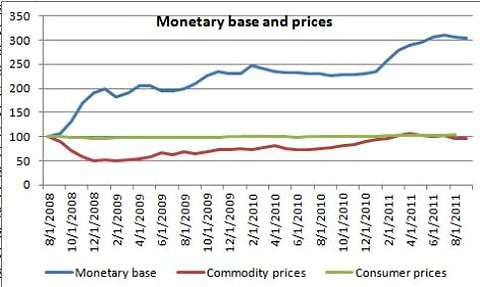
\includegraphics{img/100711krugman3-blog480.jpg}
    \caption{Entwicklung des Preises auf Basis der Geldmenge während der Finazkrise 08/09, \cite{Krugman2011}}
\end{figure}    

Eindeutig lässt sich dabei feststellen, dass obwohl die Geldmenge innerhalb der Krisenzeit, sowie auch danach, massiv auf das fast dreifache anstieg. Laut der Quantitätstheorie und der Quantitätsgleichung \vref{allg. Q-Formel} müsste also auch der durchschnittliche Preis um einen äquivalenten Faktor ansteigen. In der Grafik ist allerdings zu erkennen, dass dieser Anstieg entgegen der Prognose der Quantitätstheorie, nicht erfolgte.

\subsection{Wie erhält der Endverbaucher das Geld?}

Innerhalb der Quantitätstheorie wird oftmals in Beispielen argumentiert, dass es nicht von Relevanz ist, wie eine Geldmengenerhöhung seitens der Zentralbank zum Endverbraucher gelangt. Hierbei wird von den Vertretern dieser Theorie oftmals die in Beipsiel \vref{Bsp.kUmlauf} erwähnt Helikopteranekdote angeführt.


Diese Annahme bringt weitere Herausforderungen mit sich, da es bei weitem nicht trivial oder ohne Bedeutung ist, wie eine Geldmengenerhöhung beim Endverbraucher ankommt. Die direkteren Nutznießer einer Geldmengenerhöhung sind primär Banken und andere Finanzinstitute, sodass der Endverbraucher eher an zweiter, wenn nicht sogar dritter Stelle steht. Somit gilt es auch für diese Annahme eine Lösung zu finden, die sich im Rahmen der Theorie bewegt, welche gleichzeitig keine der anderen Annahmen verletzt oder die Einschränkung der Allgemeinegültigkeit der Theorie mit sich bringt.
\section*{Todos}

\begin{itemize}
    \item \textbf{Quellen, Quellen, Quellen}
\end{itemize}

\printbibliography[title=Literaturverzeichnis]

\end{document}

